\documentclass[]{mangos-musings}
\usepackage[dvipsnames]{xcolor}
\allowdisplaybreaks
\usepackage{array}
\usepackage{multicol}
\pagenumbering{gobble}
\begin{document}
\title{21-259 Recitation Selected Solutions \hfill \small{tylery}}
\tableofcontents

\newpage
\section*{08-26-2025}
\subsection*{Basics}
This class is \textbf{Calculus in Three Dimensions}, thus the class will require you to think in 3-D.
\begin{itemize}
  \item Get used to drawing in 3-D. 
  \\ My preference is to draw the usual vertical and horizontal axes. 
  \\ Label the horizontal axis $y$ and the vertical axis $z$. 
  \\ Then draw a diagonal from the bottom left to the top right, passing through the origin. Label this axis $x$.
  Note that you can interchange any of the axis labels as necessary (which will come in handy when we start doing 3-D integration). 
  \item In $\R^3$, the (Euclidean) distance (also referred to as the $L_2$ norm) between any two points $(x_1, y_1, z_1)$ and $(x_2, y_2, z_2)$
  is given by the formula 
  \[d = \sqrt{(x_2 - x_1)^2 + (y_2 - y_1)^2 + (z_2 - z_1)^2}\]
\end{itemize}
\subsection*{Planes and Spheres}
In this course, you will often deal with planes and spheres (e.g., spherical coordinates). 
\begin{itemize}
  \item You will learn the canonical formula for a plane later (finding it involves cross products). For now, we will find equations for planes parallel to another plane.
  \item[Ex.] Write an equation of the plane passing through point $(21, 2, 59)$ that is parallel to the $xz$-plane.
  \subitem When a plane is parallel to the $xz$-plane, it means only the $x$ and $z$ coordinates may vary. 
  \subitem Thus taking the $y$-value, we get the equation $y = 2$.
  \item[Ex.] Write an equation of the plane passing through points $(2, 125, 9), (21, 25, 9), (5, 7, 9)$ that is parallel to the $xy$-plane. 
  \subitem When a plane is parallel to the xy-plane, it means only the x and y coordinates may vary. 
  \subitem Conveniently, the $z$-value in all 3 coordinates are equal; we get the equation $z = 9$.
  \item A sphere is the set of all points in space equidistant from a fixed point, the center of
  the sphere. For center $(a, b, c)$ and radius $r$, we represent the sphere by the (``canonical'') equation: 
  \[(x-a)^2 + (y-b)^2 + (z-c)^2 = r^2\]
  \item[Ex.] Find the equation of the sphere with diameter $\overline{PQ}$ where $P = (2, -1, -3)$ and $Q = (-2, 5, -1)$.
  \subitem First, find the center, which is at the midpoint of the diameter $\overline{PQ}$:
  \[C = \left(\dfrac{2 + (-2)}{2}, \dfrac{-1 + 5}{2}, \dfrac{-3 + (-1)}{2}\right) = \left(0, 2, -2\right)\]
  \subitem Next, find the radius using the distance formula (half the length of the diameter)
  \[r = \dfrac{1}{2}\norm{\overline{PQ}} 
      = \dfrac{1}{2}\sqrt{(-2 - 2)^2 + (5 - (-1))^2 + (-1 - (-3))^2}
      = \dfrac{1}{2}\sqrt{56}
      = \sqrt{\dfrac{56}{4}}
      = \sqrt{14}\]
  \subitem Thus the sphere is given by $x^2 + (y-2)^2 + (z+2)^2 = 14$
\end{itemize}
\subsection*{Vector Notation}
Vectors are quantities with magnitude and direction. In $\R^3$, the standard unit vectors are 
\[\hat{i} = \langle1, 0, 0\rangle \quad \hat{j} = \langle0, 1, 0\rangle \quad \hat{k} = \langle0, 0, 1\rangle \]

There are several notations. Fix points in $\R^3$ $P = (0, 2, 1)$ and $Q = (2, 5, 9)$
\\ Let's represent the vector $\overrightarrow{PQ} = \langle x_Q - x_P, y_Q - y_P, z_Q - z_P\rangle$.
\begin{itemize}
  \item Component Form: $\overrightarrow{PQ} = \langle 2-0, 5-2, 9-1\rangle = \langle 2, 3, 8\rangle$
  \item Using the unit vectors: $\overrightarrow{PQ} = 2\hat{i} + 3\hat{j} + 8\hat{k}$
\end{itemize}

Ex: Consider the vectors $v = \langle 0, 2, 1\rangle$ and $u = \langle 2, 5, 9\rangle$. Find a unit vector in the direction of $3v + u$. 

You will need the following rules (taken from your textbook)
\\ 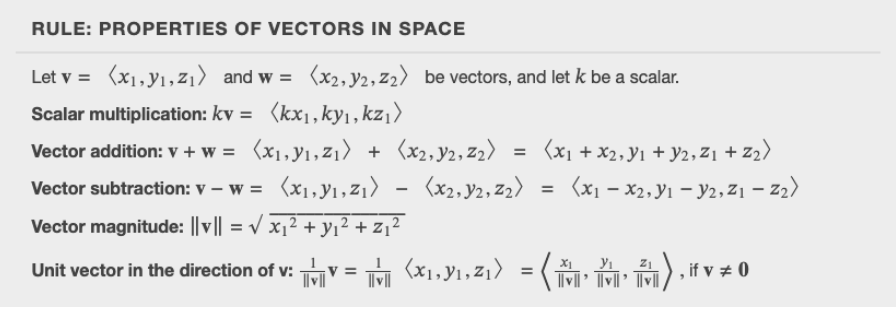
\includegraphics{assets/rec01-vectorspace.png}

Solution: first find $3v + u$, then find unit vector in that direction.
\begin{align*}
  3v + u &= \langle 3(0), 3(2), 3(1)\rangle + \langle 2, 5, 9\rangle \tag{scalar multiplication}
  \\ &=  \langle 0, 6, 3\rangle +  \langle 2, 5, 9\rangle 
  = \langle 2, 11, 12\rangle
  \\ \dfrac{1}{\norm{3v + u}} (3v + u) &= \dfrac{\langle 2, 11, 12\rangle}{\sqrt{2^2 + 11^2 + 12^2}} =  \langle \dfrac{2}{\sqrt{269}}, \dfrac{11}{\sqrt{269}}, \dfrac{12}{269}\rangle \tag{unit vector in direction}
\end{align*}
Observe that $269$ is prime, so you can't simplify the denominator. Thus we're done. Not all numbers will be pretty, but as a tip: make sure your answers are feasible. If you are taking the length of a vector with 1-digit coordinates and get a 5-digit number, that's probably wrong. 
\\ \textbf{DON'T FORGET THE SQUARE ROOT $\sqrt{}$ when taking norms!!!!}

\newpage
\subsection*{Computing 3x3 Determinants}
Useful for computing cross products. You are free to use whatever trick you want so long as you show your work. (note vertical bars means determinant, while square brackets mean matrix). 

\subsubsection*{Cofactor Method}
Key notes: $+, -, +$ (\textbf{DON'T FORGET THE MIDDLE IS NEGATIVE}) and the 2x2 sub-determinants are the elements not in the same row or column.
\begin{align*}
  \begin{vmatrix}
    a & b & c \\
    d & e & f \\ 
    g & h & i
  \end{vmatrix}
  &= a \begin{vmatrix}
    e & f \\ 
    h & i
  \end{vmatrix}
  - b \begin{vmatrix}
    d & f \\ 
    g & i
  \end{vmatrix}
  + c \begin{vmatrix}
    d & e \\ 
    g & h
  \end{vmatrix}
  = a(ei - fh) - b(di - fg) + c(dh - eg)
  \\ &= aei - afg - bdi + bfg + cdh - ceg
\end{align*}
For cross products between two vectors $u = \langle u_x, u_y, u_z \rangle$ and $v = \langle v_x, v_y, v_z \rangle$, you just compute the 3x3 determinant $\begin{vmatrix}
  \hat{i} & \hat{j} & \hat{k} \\ 
  u_x & u_y & u_z \\ 
  v_x & v_y & v_z
\end{vmatrix}$

\subsubsection*{Diagonal Method}
Recall that the 2x2 determinant is computed using the diagonals:
$\begin{vmatrix}
    a & b \\
    c & d 
\end{vmatrix} = ad - bc$, where the diagonals going from right to left are positive and diagonals going from left to right are negative. We extend this idea to 3x3 determinants:
\[\begin{vmatrix}
    a & b & c \\
    d & e & f \\ 
    g & h & i
  \end{vmatrix} \xRightarrow{expand} \begin{matrix}
    & & a & b & c & & \\
    & f & d & e & f & d & \\ 
    h & i & g & h & i & g & h
  \end{matrix} \xRightarrow{compute} aei + bfg + cdh - afh - bdi - ceg\]
which is the same result as derived from the cofactor method.



\newpage
\section*{09-02-2025}
\subsection*{Section 2.5, Checkpoint 2.47}
Find an equation of the plane containing the lines L1 and L2:
\[L1:x=-y=z\]
\[L2:\frac{x-3}{2}=y=z-2\]
\textit{On the original handout, I mistyped and had $L_2 = x - 32$. This has been corrected, as the error makes the question unsolvable since the lines would be skew.}
\subsubsection*{Worked Solution}


Let $L_1: x=-y=z = t$. The parameterized form of $L_1$ is thus $\langle t, -t, t\rangle = (0, 0, 0) + \langle 1, -1, 1\rangle t$

Let $L_2: \frac{x-3}{2}=y=z-2 = t$. The parameterized form of $L_2$ is thus $\langle2t + 3, t, t + 2 \rangle = (3, 0, 2) + \langle2, 1, 1\rangle t$.

A normal vector to the plane that contains both lines is the cross product of the two lines' direction vectors, which was $\vec{n} = \langle -2, 1, 3\rangle$ \textit{(work done in recitation)}.

Recall the equation of a plane is $\vec{n} \cdot (\vec{r} - \vec{r_0}) = 0$, where $\vec{r} = (x, y, z)$, $\vec{n}$
is a normal vector of the plane, and $\vec{r_0}$ is some arbitrary point in the plane.
\textit{Note I said \textbf{a} normal vector, since we could scale $\vec{n}$ arbitrarily.}

We have $\vec{n}$, so we just need to get $\vec{r_0}$. 
\textit{In recitation, I mentioned that we can pick any arbitrary point on either line to create the equation of the plane that contains $L_1$ and $L_2$. This holds true, and I will arbitrarily pick some points below and prove that the resulting plane equation is the same.} 
\begin{itemize}
  \item In recitation, we picked the easy point $(0, 0, 0)$, which we know to lie in $L_1$. 
  \begin{align*}
    \vec{n} \cdot (\vec{r} - \vec{r_0}) &= \langle -2, 1, 3 \rangle \cdot (x-0, y-0, z-0) 
    \\ &= -2x + y + 3z = 0
  \end{align*}
  \item But what if we had picked $(3, 0, 2)$, which was our anchor point for $L_2$?
  \begin{align*}
    \vec{n} \cdot (\vec{r} - \vec{r_0}) &= \langle -2, 1, 3 \rangle \cdot (x-3, y-0, z-2) 
    \\ &= -2(x-3) + y + 3(z-2) = 0
    \\ &= -2x + 6 + y + 3z - 6 = 0
    \\ &= -2x + y + 3z = 0 \tag{the $6$'s cancel!}
  \end{align*}
  \item As an extension, derive the plane equation you get if you choose the intersection point of $L_1$ and $L_2$! You'll see that you still reach the same plane equation.
\end{itemize}


\newpage
\section*{09-04-2025}
\textit{Note: We do NOT cover the foci of paraboloids or ellipsoids.}

\subsection*{Section 2.6, Example 2.59 Identifying Equations of Quadric Surfaces}
Identify the surfaces represented by the given equations.
\begin{enumerate}[label=(\alph*)]
  \item $16x^2 + 9y^2 + 16z^2 = 144$
  \textbf{Solution}
  Observe that all the terms are squared, and all the coefficients are positive (but not equal) so this is an ellipsoid.

  \item $9x^2 - 18x + 4y^2 + 16y - 36z + 25 = 0$

  \textbf{Solution}
  We have two squared terms, and $z$ term of degree one. We could rearrange this to get $36z = 9x^2 - 18x + 4y^2 + 16y + 25$, which appears to be a elliptic paraboloid.
\end{enumerate}

\subsection*{Section 2.6, Checkpoint 2.54}
Identify the surface represented by the equation $9x^2 + y^2 - z^2 + 2z - 10 = 0$.

\textbf{Solution} We have three squared terms, two positive coefficients and one negative coefficient. So this is a double cone.

\subsection*{Section 2.6, Exercise 350}
Find the equation of the quadric surface with points $P(x,y,z)$ that are equidistant from point $Q(0,2,0)$ and plane of equation $y=-2$. Identify the surface. 

\textbf{Solution} First, the distance from a point $(x, y, z)$ to the plane $y = -2$ is just $\abs{y}$. \textit{This is because the plane $y = -2$ has normal vector $\hat{j}$; projecting $\overrightarrow{PQ}$ onto $\hat{j}$ just yields the $y$ component.}

To do this, we want $\langle x, y, z \rangle$ that satisfies
\begin{align*}
  \sqrt{(x-0)^2 + (y-2)^2 + (z-0)^2} &= y - (-2) 
  \\ \sqrt{x^2 + (y-2)^2 + z^2} &= y + 2
  \\ x^2 + (y-2)^2 + z^2 &= (y+2)^2
  \\ x^2 + y^2 - 4y + 4 + z^2 &= y^2 + 4y + 4
  \\ x^2 + z^2 &= 8y
\end{align*}
This is the form of an elliptic paraboloid.

\newpage
\section*{09-09-2025}
\subsection*{Section 3.1, Exercise 8}
Find the limit of the following vector valued function at the indicated value of $t$.
\[\lim_{t\to 4}\left\langle \sqrt{t-3}, \dfrac{\sqrt{t} - 2}{t-4}, \tan\left(\dfrac{\pi}{t}\right)\right\rangle\]
\textbf{Solution} We can just substitute for the $x$ and $z$ components. The middle one requires more thought; direct substitution gives $\frac{0}{0}$, so we apply L'Hopital's rule.
\[\lim_{t\to 4} \dfrac{\sqrt{t}-2}{t-4} = \lim_{t\to 4} \dfrac{\frac{1}{2\sqrt{t}}}{1} = \dfrac{1}{4}\]
So the limit is 
\[\left\langle1, \dfrac{1}{4}, 1\right\rangle\]



\begin{center}
  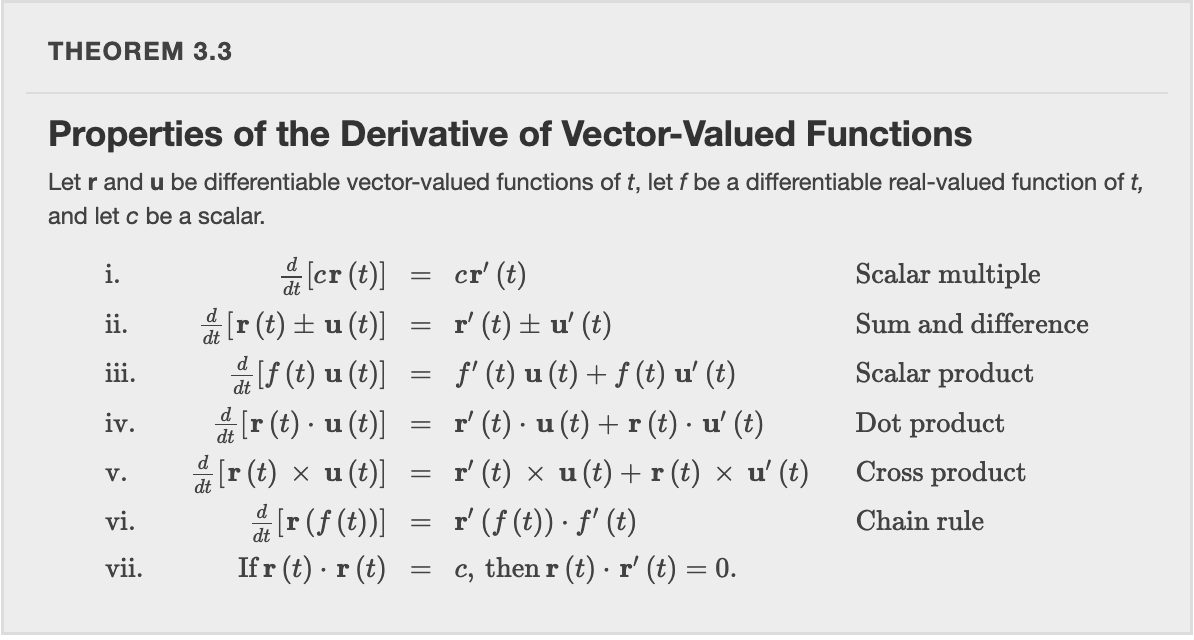
\includegraphics[scale=0.6]{assets/rec05-derivative-properties.png}
\end{center}


\newpage
\section*{10-02-2025}
Given $z = f(x, y)$ is continuous and differentiable on a closed, bounded set $D$, the strategy to find absolute extrema of $f$ on $D$ is to 
\begin{enumerate}
  \item Determine the critical points of $f$ in $D$
  \item Calculate $f$ at each of these critical points
  \item Determine the maximum and minimum values of $f$ on the boundary of its domain 
  \item Find the absolute maximum and minimum values of $f$ by comparing the values from steps 2 and 3.
\end{enumerate}




\newpage
\section*{10-07-2025 - Midterm 2 tomorrow}
Use the method of Lagrange Multipliers to find the maximum and minimum values of the function subject to the given constraints.
\subsection*{Section 4.8, Exercise 369}
Minimize $f(x, y) = x^2 + y^2$ on the hyperbola $xy = 1$.

\textbf{Solution} Our objective is $f$, and our constraint is $g(x, y) = xy = 1$.
\begin{align*}
  \nabla f &= \lambda \nabla g(x, y)
  \\ (2x, 2y) &= \lambda (y, x)
\end{align*}
So our system to solve is 
$\begin{cases}
  (1) & 2x = \lambda y 
  \\ (2) & 2y = \lambda x 
  \\ (3) & xy = 1
\end{cases}$ which we do by solving for $\lambda$:
\begin{align*}
  \lambda &= \frac{2y}{x} \tag{from eqn. (2)}
  \\ 2x &= \frac{2y^2}{x} \tag{from subst. into eqn. (1)}
  \\ 2x^2 &= 2y^2 
  \\ x &= \pm y
\end{align*}
Combine $x = \pm y$ with $xy = 1$, we get $(x, y) = (1, 1)$ or $(x, y) = (-1, -1)$. A quick intuition check; a hyperbola $xy = 1$ will have asymptotes along the $x$ and $y$ axes. 
And note as $x$ or $y$ goes to infinity, $x^2 + y^2$ also goes to infinity. So clearly the points we have solved for can't be the maximums, so they're probably the minimums. Graphing $xy = 1$ on Desmos reveals that our answer makes sense:
\[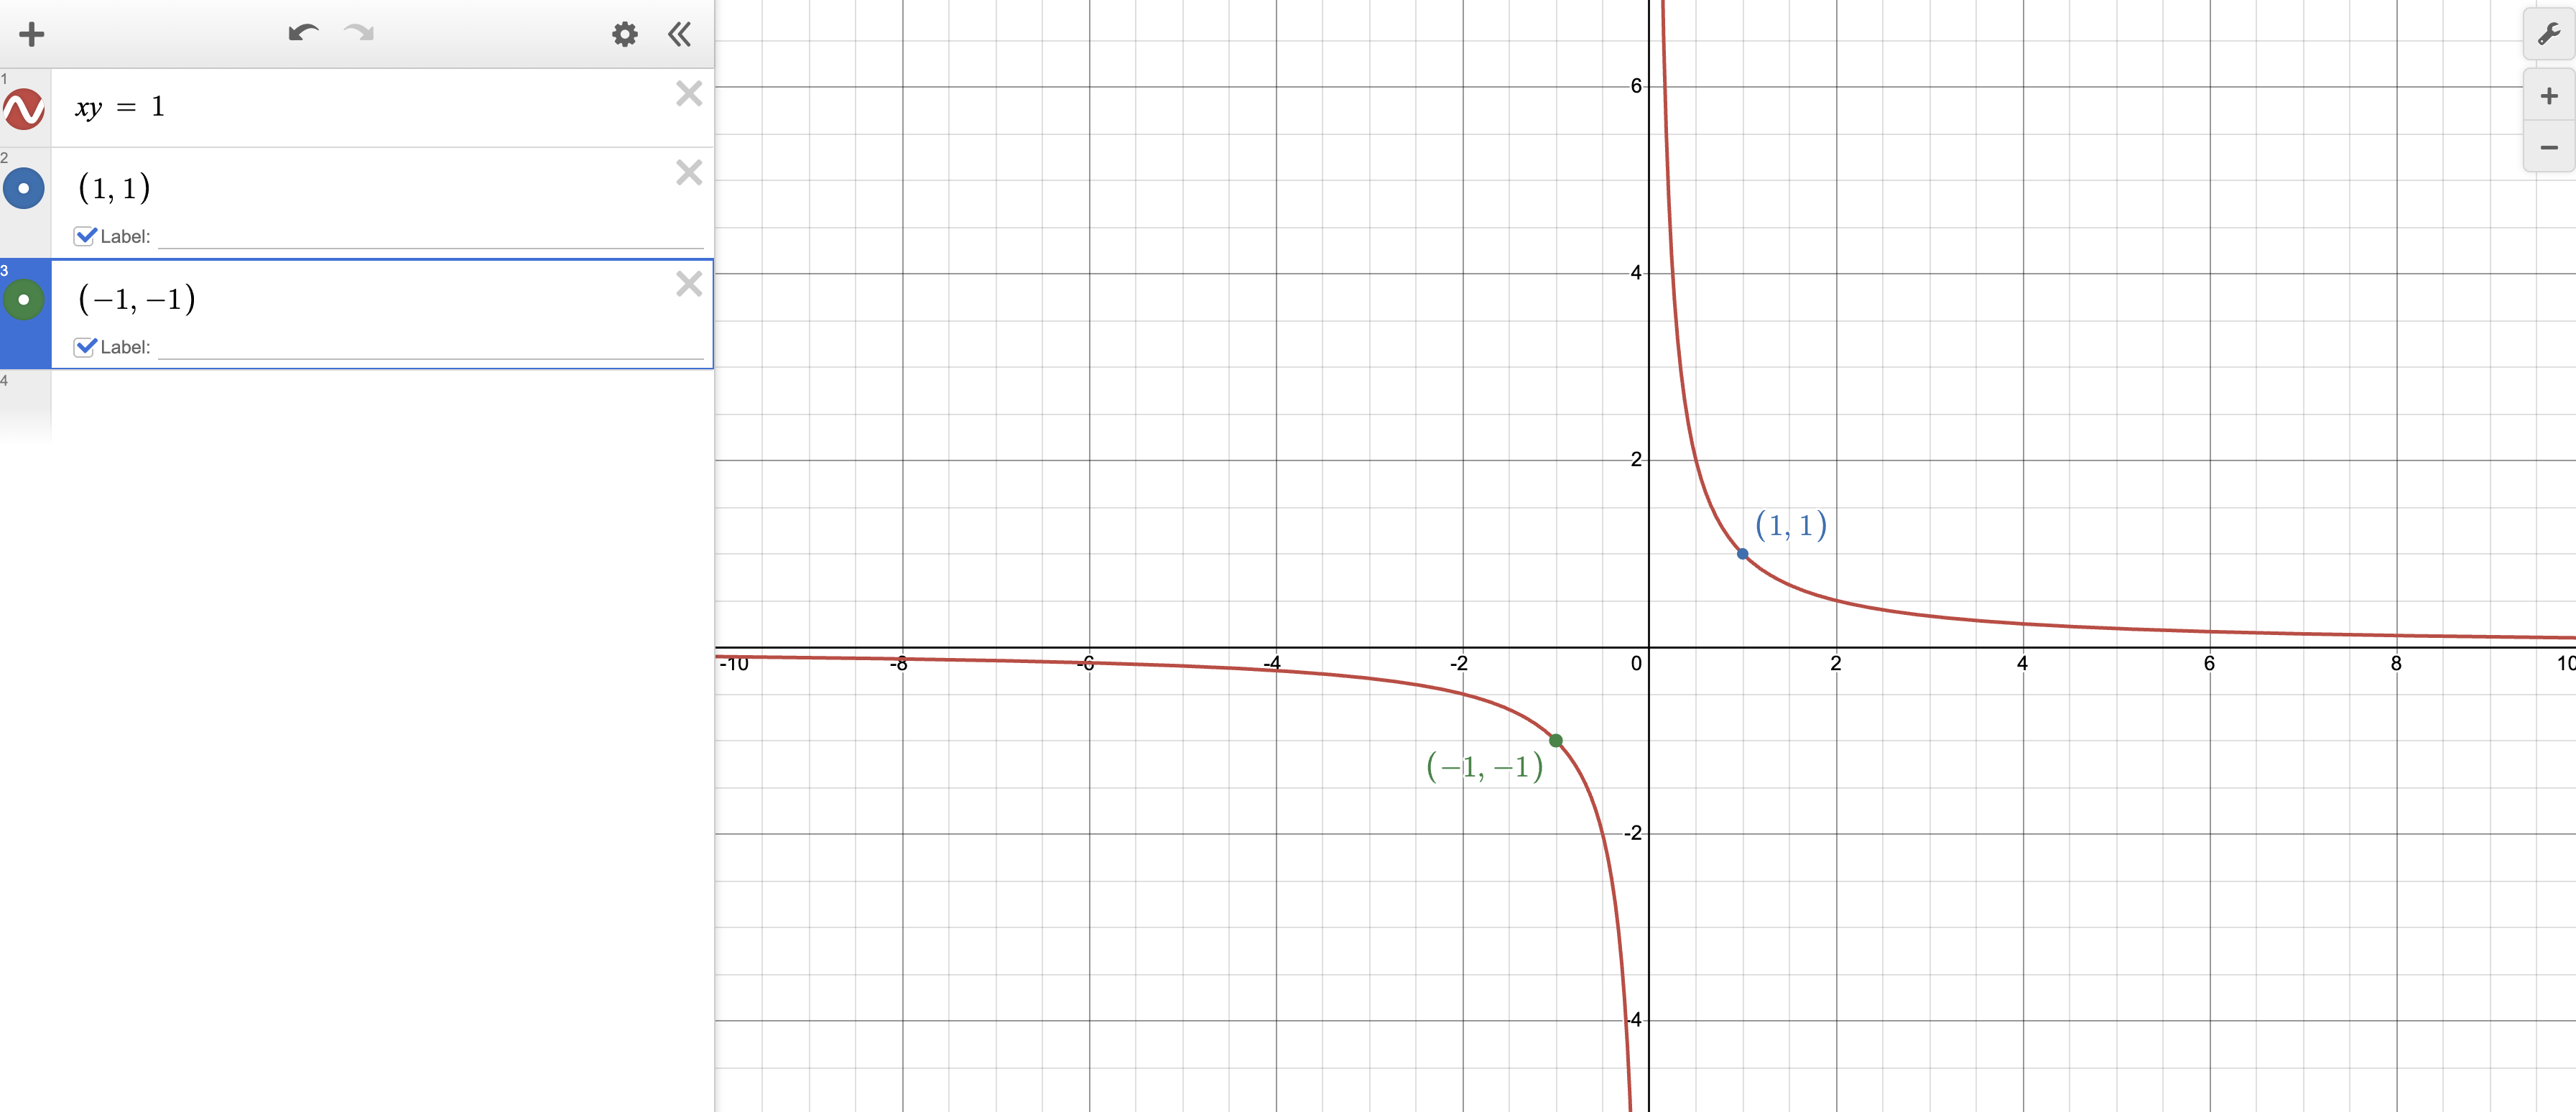
\includegraphics[scale=0.2]{assets/rec13.1.png}\]

% \newpage
% \subsection*{Section 4.8, Exercise 373}
% The curve $x^3 - y^3 = 1$ is asymptotic to the line  $y = x$. 
% Find the point(s) on the curve $x^3 - y^3 = 1$ 
% farthest from the line $y = x$.

% \textit{What is the function we seek to minimize?}
% \begin{align*}
%   \\ \\ \\
% \end{align*}
\newpage
\subsection*{Section 4.8, Exercise 374}
Maximize $U(x, y) = 8x^{\frac{4}{5}} y^{\frac{1}{5}}$ under constraint $4x + 2y = 12$.

\textbf{Solution} We solve for $y$ in terms of $x$, then treat this as a calc 1 optimization problem.
\textit{The arithmetic might not be right, please let me know if this is incorrect. The approach is sound though.}
\begin{align*}
  4x + 2y = 12 & \implies 2x + y = 6
  \\ & \implies y = 6 - 2x 
  \\ & \implies U(x) = 8x^{4/5}\cdot (6 - 2x)
\end{align*}
Now we maximize using calc 1 techniques:
\begin{align*}
  \frac{dU}{dx} &= 8 \cdot\left( \frac{4}{5}x^{-1/5} \cdot (6 - 2x) + (-2)\cdot 8x^{4/5}\right) = 0
  \\ &\implies \frac{4}{5}x^{-1/5} \cdot (6 - 2x) + (-2)\cdot 8x^{4/5} = 0
  \\ &\implies 16x^{4/5} = \frac{24}{5}x^{-1/5} - \frac{8}{5}x^{4/5}
  \\ &\implies \frac{72}{5}x^{4/5} = \frac{24}{5}x^{-1/5}
  \\ &\implies 3x^{4/5} = x^{-1/5}
  \\ &\implies 3x = 1 \implies x = \frac{1}{3} \implies y = 6 - 2x = \frac{16}{3}
\end{align*}
Now is this is a max or min?
\begin{align*}
  \frac{dU}{dx} &= \frac{32}{5}x^{-1/5} \cdot (6 - 2x) -16\cdot 8x^{4/5} = \frac{192}{5}x^{-1/5} - \frac{64}{5}x^{4/5} - 128 x^{4/5} = \frac{192}{5}x^{-1/5} - \frac{704}{5}x^{4/5}
  \\ \frac{d^2U}{dx^2} &= -\frac{192}{25}x^{-6/5} - \frac{2816}{25}x^{-1/5}
\end{align*}
If we evaluate the second derivative at $x =1/3, y = 16/3$, it's a little ugly, but we'll see that since $x$ is positive, $x^{-6/5}, x^{-1/5}$ are both positive, and notice the coefficients are both negative, so the overall second derivative is negative at the point we found. Therefore, $U\left(\frac{1}{3}, \frac{16}{3}\right)$ is a maximum, and we just plug in to find the value.

\newpage
\subsection*{Section 4.8, Exercise 379}
Maximize $f(x, y, z) = x^2 + y^2 + z^2$ under constraints $x + y + z = 9$ and $x + 2y + 3z = 20$.

\textbf{Solution} Objective is $f$, constraints $g_1$, $g_2$. Lagrange multipliers gives us 
\begin{align*}
  \nabla f &= \lambda \cdot \nabla g_1 + \mu \cdot \nabla g_2
  \\ (2x, 2y, 2z) &= (\lambda, \lambda, \lambda) + (\mu, 2\mu, 3\mu)
\end{align*}
So our system is:
$\begin{cases}
  (1) & 2x = \lambda + \mu
  \\ (2) & 2y = \lambda + 2\mu  
  \\ (3) & 2z = \lambda + 3\mu 
  \\ (4) & x + y + z = 9
  \\ (5) & x + 2y + 3z = 20
\end{cases}$
\begin{align*}
  & 2x + 2y + 2z = 3\lambda + 6\mu = 18 \tag{eqns. 1, 2, 3, 4} \\
  \implies & \lambda = 6 - 2\mu \\ 
  \implies & 2y = 6 - 2\mu + 2\mu = 6 \implies y = 3 \tag{eqn. 2}\\
  \implies & x + z = 6 \cap x + 3z = 14 \tag{eqns. 4, 5}\\
  \implies & 2x = 8 \implies z = 4 \implies x = 2
\end{align*}
So we've found the solution $(x, y, z) = (2, 3, 4), f(2, 3, 4) = 29$, but this is a minimum, so there is no maximum. 

Think of it this way, our constraints are two intersecting planes so our solution space is a line. The function we maximize is the distance from the origin, squared. Therefore, there are points along this line infinitely far from the origin, so the point we made is probably the minimum of $f$ under these constraints. Graphing shows us this intuition is correct:
\[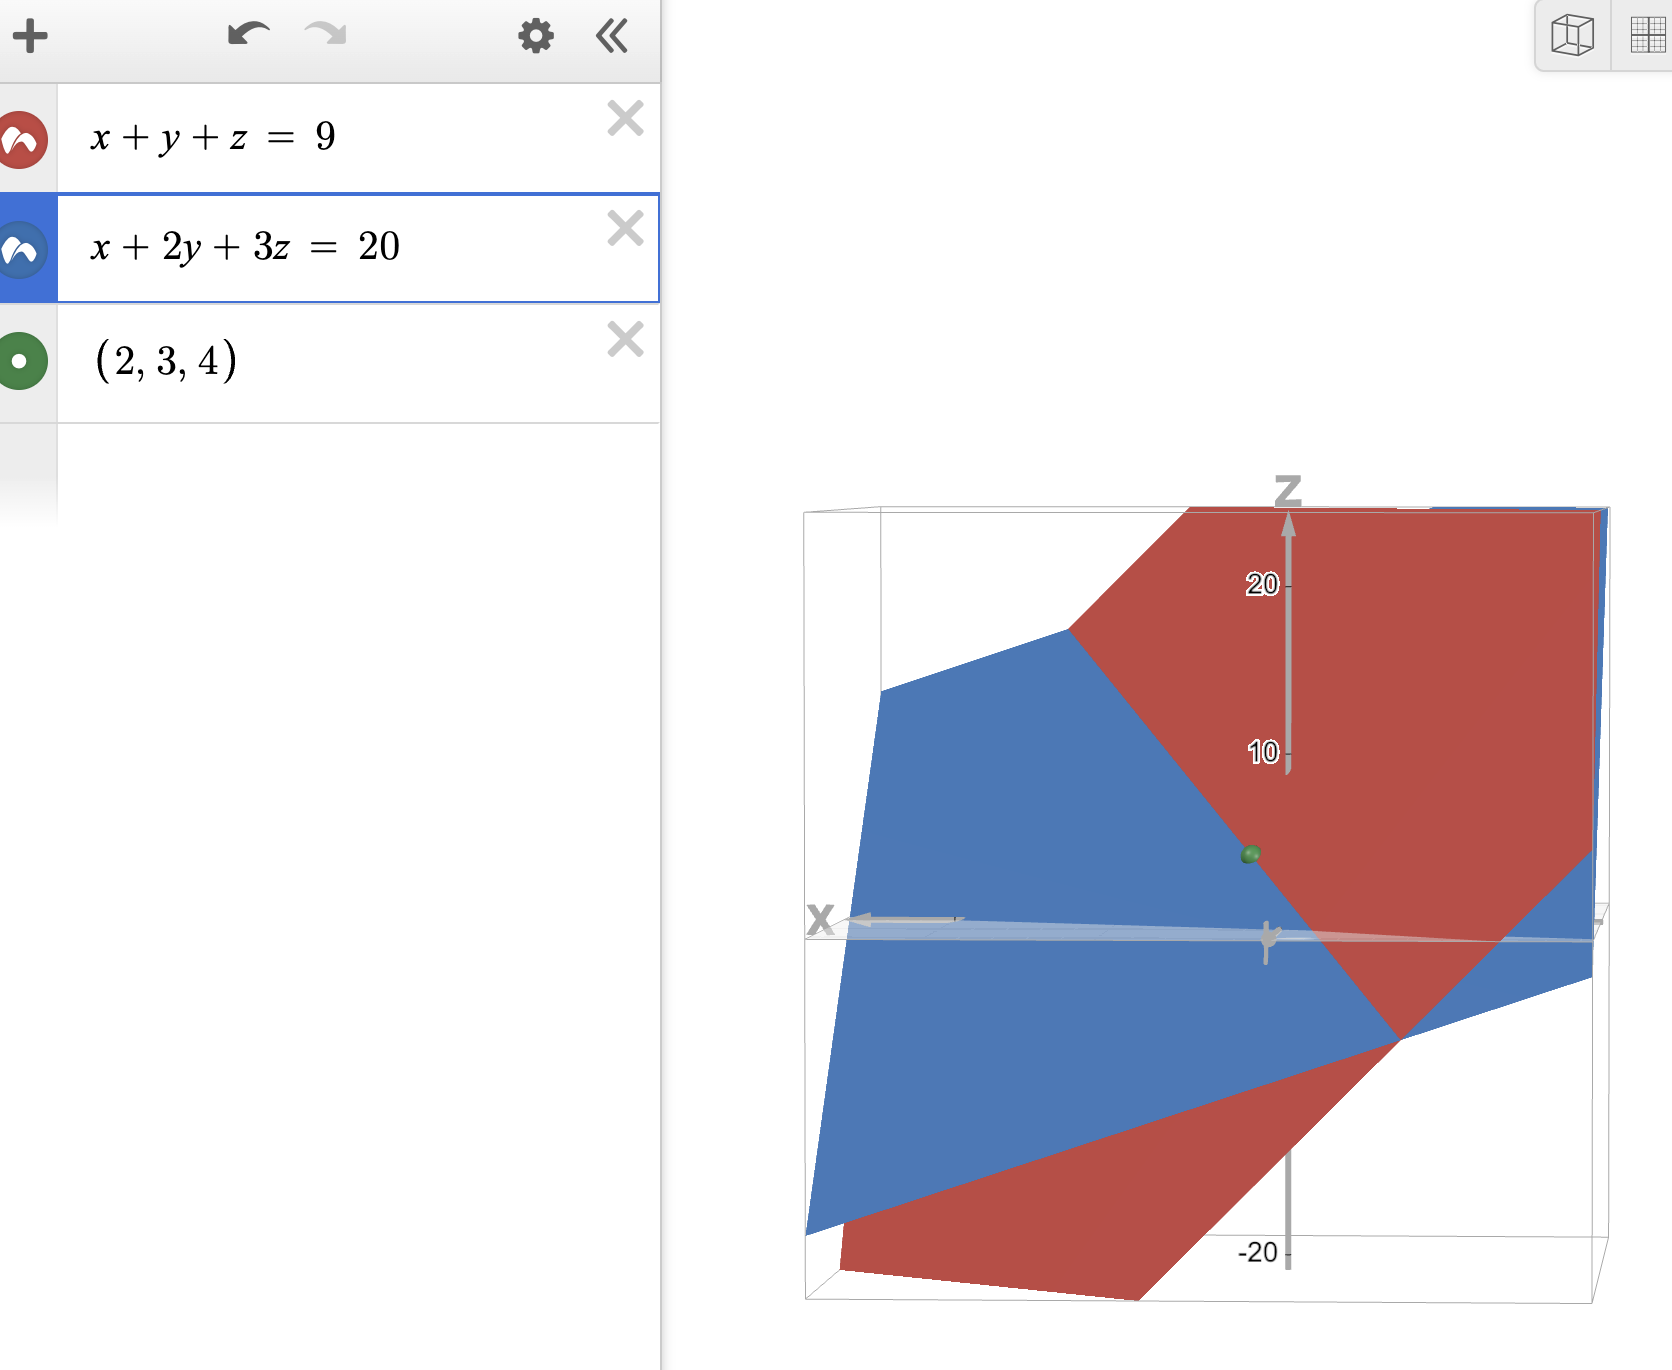
\includegraphics[scale=0.3]{assets/rec13.4.png}\]


% \newpage
% \subsection*{Section 4.8, Exercise 388}
% A large container in the shape of a rectangular solid must have a volume of $480 m^3$. The bottom of the container costs $\$5/m^2$ to construct, whereas the top and sides cost $\$3 /m^2$ to construct. Use Lagrange multipliers to find the dimensions of the container of this size that has the minimum cost.

% \textbf{Solution} Let $x$ be the length, $y$ the width, $z$ the height. Thus, the bottom and top have area $xy$, the sides have area $yz$, and the front and back have area $xz$. Objective is a cost function $C(x, y, z) = 5xy + 3xy + 3yz + 3yz + 3xz + 3xz = 8xy + 6yz + 6xz$. Constraint is $V(x, y, z) = xyz = 480$.
% \begin{align*}
%   \nabla C &= \lambda \nabla V 
%   \\ (8y + 6z, 8x + 6z, 6x + 6y) &= (\lambda yz, \lambda xz, \lambda xy)
% \end{align*}
% So our system is $\begin{cases}
%   (1) & 8y + 6z = \lambda yz\\
%   (2) & 8x + 6z = \lambda xz\\ 
%   (3) & 6x + 6y = \lambda xy\\ 
%   (4) & xyz = 480\\ 
% \end{cases}$

% \textit{In recitation, I mistakenly solved for a solution where $z = 0$. That's actually not possible because of eqn. 4}
% \begin{align*}
%   & \lambda = \frac{8y + 6z}{yz} = \frac{8x + 6z}{xz} \tag{eqns. 1, 2} \\ 
%   \implies & 8xyz + 6xz^2 = 8xyz + 6yz^2 \implies 6xz^2 = 6yz^2 \implies x = y \\ 
%   \implies & 12x = \lambda x^2 \tag{eqn. 3} \\ 
%   \implies & x = 12 \land y = 12 \tag{since $x\neq 0$ by constraint 4} \\ 
%   \implies & z = \frac{480}{12 \cdot 12} = \frac{40}{12} = \frac{10}{3}
% \end{align*}
% So we plugin to get $C(12, 12, \frac{10}{3}) = 8 \cdot 144 + 6\cdot 12 \cdot \frac{10}{3} + 6\cdot 12 \cdot \frac{10}{3} = 1152 + 480 = 1632$. But is this a maximizing or minimizing cost?

% Well it's probably maximizing (when a box is roughly a square box, surface area is maximized), so this is unfortunately not the correct solution.

% To minimize, we do the same process but we try a different set of equations. I just used a lagrange multipliers calculator and got


\newpage
\section*{10-09-2025 - Post Midterm 2, No Content}

\newpage
\section*{10-21-2025}

\newpage
\section*{10-23-2025}

\newpage
\section*{10-28-2025}

\newpage
\section*{10-30-2025}

\newpage
\section*{11-06-2025}

\newpage
\section*{11-11-2025 - Midterm 3 tomorrow}

\newpage
\section*{11-13-2025 - Post Midterm 3, No Content}

\newpage
\section*{11-18-2025}

\newpage
\section*{11-20-2025}

\newpage
\section*{11-25-2025}

\newpage
\section*{12-02-2025 - Final Review}

\newpage
\section*{12-04-2025 - Final Review}
\end{document}